\section{Сверточные нейронные сети}

\subsection{Архитектура}

Большая часть современных нейронных сетей направленных на анализ изображений базируются на архитектуре сверточной нейронной сети.
Ранние нейронные сети состояли из полносвязных слоев - слоев, в которых каждый нейрон связан с каждым нейроном следующего слоя, что значительно увеличивало вычислительную сложность системы при увеличении количества нейронов. 
В типовых сверточных нейронных сетях преимущественно используются сверточные слои. 

Сверточные слои характеризуются использованием матриц весов, называемых фильтрами или ядрами, которые обладают размерностью меньше исходных данных. Такое ядро с определенным шагом проходит по набору входных данных $(I)$ и вычисляет суммы произведений соответствующих значений ячеек и весов, формируя карту признаков $(I * K)$. Один сверточный слой может содержать несколько ядер и соответственно несколько карт признаков.

\begin{figure}[H]
\centering
\begin{tikzpicture}[scale=0.8,  every node/.style={scale=0.8}]

	\matrix (mtr) [matrix of nodes,row sep=-\pgflinewidth, nodes={draw}]
	{
		0 & 1 & 1 & |[fill=red!30]| 1 & |[fill=red!30]| 0 & |[fill=red!30]| 0 & 0\\
		0 & 0 & 1 & |[fill=red!30]| 1 & |[fill=red!30]| 1 & |[fill=red!30]| 0 & 0\\
		0 & 0 & 0 & |[fill=red!30]| 1 & |[fill=red!30]| 1 & |[fill=red!30]| 1 & 0\\
		0 & 0 & 0 & 1 & 1 & 0 & 0\\
		0 & 0 & 1 & 1 & 0 & 0 & 0\\
		0 & 1 & 1 & 0 & 0 & 0 & 0\\
		1 & 1 & 0 & 0 & 0 & 0 & 0\\
	};

	\draw[very thick, red] (mtr-1-4.north west) rectangle (mtr-3-6.south east);

	\matrix (K) [right=0.2em of mtr,matrix of nodes,row sep=-\pgflinewidth, nodes={draw, fill=blue!30}]
	{
		1 & 0 & 1 \\
		0 & 1 & 0 \\
		1 & 0 & 1 \\
	};

	\matrix (ret) [right=0.2em of K,matrix of nodes,row sep=-\pgflinewidth, nodes={draw}]
	{
		1 & 4 & 3 & |[fill=green!30]| 4 & 1\\
		1 & 2 & 4 & 3 & 3\\
		1 & 2 & 3 & 4 & 1\\
		1 & 3 & 3 & 1 & 1\\
		3 & 3 & 1 & 1 & 0\\
	};

	\draw[very thick, green] (ret-1-4.north west) rectangle (ret-1-4.south east);

	\draw[densely dotted, blue, thick] (mtr-1-4.north west) -- (K-1-1.north west);
	\draw[densely dotted, blue, thick] (mtr-3-4.south west) -- (K-3-1.south west);
	\draw[densely dotted, blue, thick] (mtr-1-6.north east) -- (K-1-3.north east);
	\draw[densely dotted, blue, thick] (mtr-3-6.south east) -- (K-3-3.south east);

	\draw[densely dotted, green, thick] (ret-1-4.north west) -- (K-1-1.north west);
	\draw[densely dotted, green, thick] (ret-1-4.south west) -- (K-3-1.south west);
	\draw[densely dotted, green, thick] (ret-1-4.north east) -- (K-1-3.north east);
	\draw[densely dotted, green, thick] (ret-1-4.south east) -- (K-3-3.south east);

	\matrix (K) [right=0.2em of mtr,matrix of nodes,row sep=-\pgflinewidth, nodes={draw, fill=blue!10}]
	{
		1 & 0 & 1 \\
		0 & 1 & 0 \\
		1 & 0 & 1 \\
	};

	\draw[very thick, blue] (K-1-1.north west) rectangle (K-3-3.south east);
\end{tikzpicture}
\caption{Операция свертки} \label{convolution}
\end{figure}

Так как признаки уже обнаружены, для упрощения дальнейших вычислений можно снизить детализацию входных данных. Это обеспечивает субдискретизирующий (пулинговый) слой, уменьшая размерность входных карт признаков: из нескольких соседних нейронов берется максимальное или среднее значение, тем самым формируя нейрон карты признаков меньшей размерности. Это позволяет снизить количество параметров, используемых в дальнейших вычислениях сети. 

\begin{figure}[H]
    \centering
    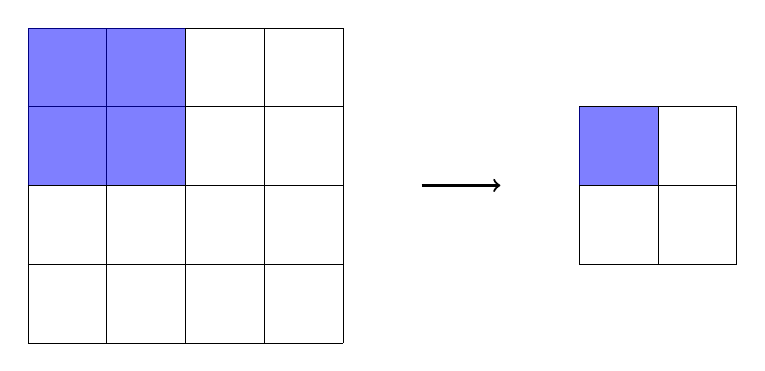
\begin{tikzpicture}
        \draw[step=1cm,very thin] (-2,-2) grid (2,2);
        \fill[blue, opacity=0.5] (0,2) rectangle (-2,0);
        \draw[thick,->] (3,0) -- (4,0) node[anchor=north west] {};
        \draw[step=1cm,very thin] (5,-1) grid (7,1);
        \fill[blue, opacity=0.5] (5,0) rectangle (6,1);
    \end{tikzpicture}
    \caption{Субдискретизация} \label{pooling}
\end{figure}

Сверточная нейронная сеть может иметь несколько пар чередующихся сверточных и субдискретизирующих слоев. 
Таким образом, на примере изображений, на начальных слоях сеть находит такие простейшие признаки как границы и углы. Затем, по мере углубления в сеть, определяются всё более сложные конструкции: от простейших фигур до целых классов, независимо от их местоположения на изображении. Завершается сеть стандартными полносвязными слоями которые сопоставляют полученные карты признаков какому-либо классу.  


\subsection{AlexNet}

\subsection{VGG-16}

\subsection{GoogLeNet}

\subsection{ResNet}

\clearpage